\documentclass{article}
\title{The profile2 data}
\usepackage{graphicx}
\usepackage{Statweave}
\begin{document}
\maketitle
The data:
\begin{verbatim}
bellydancer 7 10 6 5 
bellydancer 8 9 5 7 
bellydancer 5 10 5 8 
bellydancer 6 10 6 8 
bellydancer 7 8 7 9 
politician  4 4 4 4 
politician 6 4 5 3 
politician 5 5 5 6  
politician 6 6 6 7  
politician 4 5 6 5 
admin 3 1 1 2 
admin 5 3 1 5 
admin 4 2 2 5 
admin 7 1 2 4 
admin 6 3 3 3 
\end{verbatim}
The SAS code and output:
\begin{Winput}
options linesize=80;

data profile;
  infile "profile.dat";
  input group $ read dance tv ski;

proc discrim can list out=fred;
  class group;

proc print;

proc gplot;
  plot Can1*Can2=group;

run;
\end{Winput}
\begin{Woutput}
The DISCRIM Procedure
Total Sample Size       15          DF Total                14
Variables                4          DF Within Classes       12
Classes                  3          DF Between Classes       2

Number of Observations Read             15
Number of Observations Used             15

                          Class Level Information
            Variable                                                  Prior
group       Name        Frequency       Weight    Proportion    Probability
admin       admin               5       5.0000      0.333333       0.333333
bellydan    bellydan            5       5.0000      0.333333       0.333333
politici    politici            5       5.0000      0.333333       0.333333

Pooled Covariance Matrix Information
               Natural Log of the
 Covariance    Determinant of the
Matrix Rank     Covariance Matrix
          4               0.38667

The DISCRIM Procedure
Pairwise Generalized Squared Distances Between Groups
 2         _   _       -1  _   _
D (i|j) = (X - X )' COV   (X - X )
            i   j           i   j

      Generalized Squared Distance to group
From
group            admin      bellydan      politici
admin                0      77.68532      25.14460
bellydan      77.68532             0      27.90946
politici      25.14460      27.90946             0

The DISCRIM Procedure
Canonical Discriminant Analysis
                              Adjusted    Approximate        Squared
              Canonical      Canonical       Standard      Canonical
            Correlation    Correlation          Error    Correlation
       1       0.970481       0.963344       0.015545       0.941834
       2       0.814155       0.798467       0.090107       0.662849
                           Eigenvalues of Inv(E)*H
                             = CanRsq/(1-CanRsq)
            Eigenvalue    Difference    Proportion    Cumulative
       1       16.1922       14.2262        0.8917        0.8917
       2        1.9660                      0.1083        1.0000
                  Test of H0: The canonical correlations in the
                    current row and all that follow are zero
            Likelihood    Approximate
                 Ratio        F Value    Num DF    Den DF    Pr > F
       1    0.01961069          13.82         8        18    <.0001
       2    0.33715124           6.55         3        10    0.0100

The DISCRIM Procedure
Canonical Discriminant Analysis
         Total Canonical Structure
Variable              Can1              Can2
read              0.501543         -0.326770
dance             0.988676         -0.137490
tv                0.870725          0.447979
ski               0.762946         -0.153062

        Between Canonical Structure
Variable              Can1              Can2
read              0.877480         -0.479613
dance             0.993263         -0.115878
tv                0.918130          0.396278
ski               0.986131         -0.165969

     Pooled Within Canonical Structure
Variable              Can1              Can2
read              0.145376         -0.228037
dance             0.922261         -0.308780
tv                0.537024          0.665194
ski               0.278589         -0.134560

The DISCRIM Procedure
Canonical Discriminant Analysis
Total-Sample Standardized Canonical Coefficients
Variable              Can1              Can2
read           0.018261344      -0.668274819
dance          3.112399048      -1.508589983
tv             0.939269988       2.465444147
ski           -0.085702316      -0.419490983

Pooled Within-Class Standardized Canonical Coefficients
Variable              Can1              Can2
read           0.016411781      -0.600589963
dance          0.869166285      -0.421287737
tv             0.396721290       1.041334435
ski           -0.061140572      -0.299267509

         Raw Canonical Coefficients
Variable              Can1              Can2
read           0.012974652      -0.474808056
dance          0.952123961      -0.461497594
tv             0.474172636       1.244632708
ski           -0.041536839      -0.203312237

     Class Means on Canonical Variables
group                 Can1              Can2
admin         -4.347308175      -0.922471653
bellydan       4.466326504      -0.850639955
politici      -0.119018329       1.773111608

The DISCRIM Procedure
Linear Discriminant Function
               _     -1 _                              -1 _
Constant = -.5 X' COV   X      Coefficient Vector = COV   X
                j        j                                 j

      Linear Discriminant Function for group
Variable         admin      bellydan      politici
Constant     -12.19602     -74.39378     -31.10485
read           3.13549       3.21574       1.91047
dance          1.91503      10.27355       4.69688
tv            -0.20061       4.06798       5.15934
ski            1.38042       0.99973       0.65675

The DISCRIM Procedure
Classification Results for Calibration Data: WORK.PROFILE
Resubstitution Results using Linear Discriminant Function
Generalized Squared Distance Function
 2         _       -1   _
D (X) = (X-X )' COV  (X-X )
 j          j            j
Posterior Probability of Membership in Each group
                   2                    2
Pr(j|X) = exp(-.5 D (X)) / SUM exp(-.5 D (X))
                   j        k           k

          Posterior Probability of Membership in group
       From        Classified
Obs    group       into group       admin    bellydan    politici
  1    bellydan    bellydan        0.0000      1.0000      0.0000
  2    bellydan    bellydan        0.0000      1.0000      0.0000
  3    bellydan    bellydan        0.0000      1.0000      0.0000
  4    bellydan    bellydan        0.0000      1.0000      0.0000
  5    bellydan    bellydan        0.0000      0.9973      0.0027
  6    politici    politici        0.0028      0.0000      0.9972
  7    politici    politici        0.0001      0.0000      0.9999
  8    politici    politici        0.0000      0.0000      1.0000
  9    politici    politici        0.0000      0.0021      0.9979
 10    politici    politici        0.0000      0.0000      1.0000
 11    admin       admin           1.0000      0.0000      0.0000
 12    admin       admin           1.0000      0.0000      0.0000
 13    admin       admin           1.0000      0.0000      0.0000
 14    admin       admin           1.0000      0.0000      0.0000
 15    admin       admin           0.9821      0.0000      0.0179

The DISCRIM Procedure
Classification Summary for Calibration Data: WORK.PROFILE
Resubstitution Summary using Linear Discriminant Function
Generalized Squared Distance Function
 2         _       -1   _
D (X) = (X-X )' COV  (X-X )
 j          j            j
Posterior Probability of Membership in Each group
                   2                    2
Pr(j|X) = exp(-.5 D (X)) / SUM exp(-.5 D (X))
                   j        k           k

   Number of Observations and Percent Classified into group
From
group           admin      bellydan      politici        Total
admin               5             0             0            5
               100.00          0.00          0.00       100.00
bellydan            0             5             0            5
                 0.00        100.00          0.00       100.00
politici            0             0             5            5
                 0.00          0.00        100.00       100.00
Total               5             5             5           15
                33.33         33.33         33.33       100.00
Priors        0.33333       0.33333       0.33333

              Error Count Estimates for group
                   admin    bellydan    politici       Total
Rate              0.0000      0.0000      0.0000      0.0000
Priors            0.3333      0.3333      0.3333

                                                      b       p
                                                      e       o
                                                      l       l       _
      g        d                              a       l       i       I
      r     r  a         C        C    C C    d       y       t       N
 O    o     e  n   s     a        a    a a    m       d       i       T
 b    u     a  c t k     n        n    n n    i       a       c       O
 s    p     d  e v i     1        2    3 4    n       n       i       _
 1 bellydan 7 10 6 5  5.23731 -0.58059 . . 0.00000 1.00000 0.00000 bellydan
 2 bellydan 8  9 5 7  3.74092 -2.24515 . . 0.00000 1.00000 0.00000 bellydan
 3 bellydan 5 10 5 8  4.61258 -1.48554 . . 0.00000 1.00000 0.00000 bellydan
 4 bellydan 6 10 6 8  5.09973 -0.71571 . . 0.00000 1.00000 0.00000 bellydan
 5 bellydan 7  8 7 9  3.64109  0.77379 . . 0.00000 0.99729 0.00271 bellydan
 6 politici 4  4 4 4 -1.42116  1.32687 . . 0.00283 0.00000 0.99717 politici
 7 politici 6  4 5 3 -0.87950  1.82520 . . 0.00008 0.00000 0.99992 politici
 8 politici 5  5 5 6 -0.06496  1.22857 . . 0.00001 0.00000 0.99998 politici
 9 politici 6  6 6 7  1.33277  1.33359 . . 0.00000 0.00214 0.99786 politici
10 politici 4  5 6 5  0.43777  3.15133 . . 0.00000 0.00000 1.00000 politici
11 admin    3  1 1 2 -5.62995 -0.14110 . . 1.00000 0.00000 0.00000 admin
12 admin    5  3 1 5 -3.82437 -2.62365 . . 1.00000 0.00000 0.00000 admin
13 admin    4  2 2 5 -4.31529 -0.44271 . . 0.99999 0.00000 0.00001 admin
14 admin    7  1 2 4 -5.18696 -1.20233 . . 1.00000 0.00000 0.00000 admin
15 admin    6  3 3 3 -2.77997 -0.20257 . . 0.98209 0.00000 0.01791 admin
\end{Woutput}
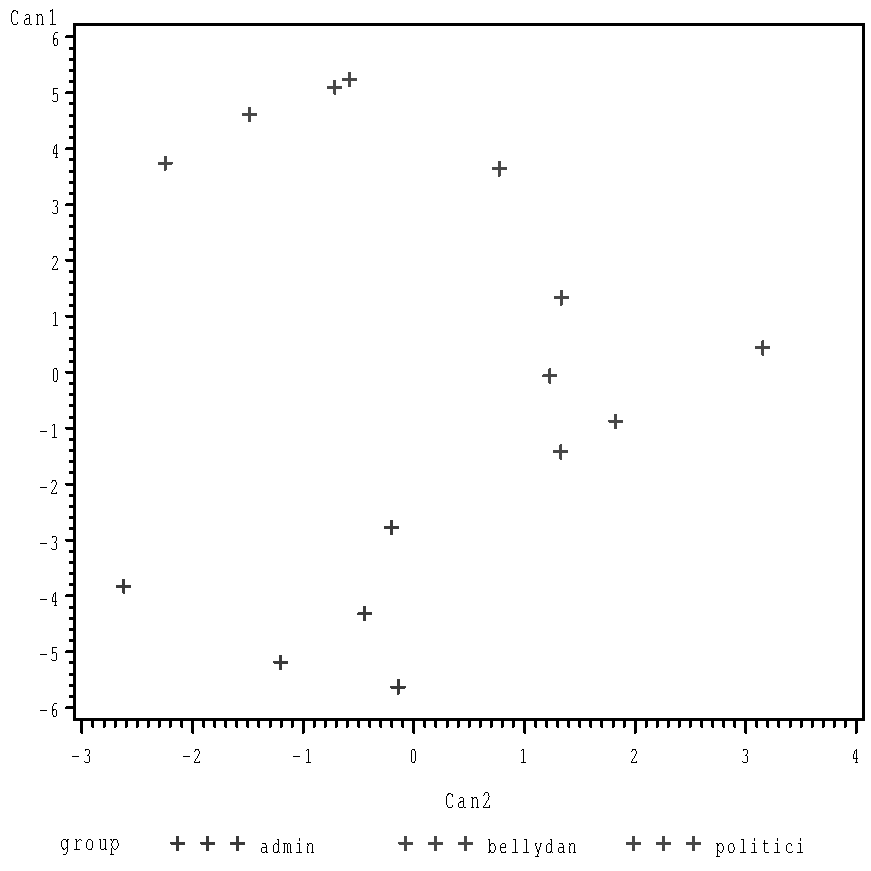
\includegraphics[]{profile2-1-SAS-fig.pdf}
\end{document}
